
\chapter{Examining Model Behavior}
\label{chap:investigating}

In this chapter, we observe behaviors of neural \acp{lm} in specific \ac{d2t} generation scenarios, building upon custom datasets.

In \autoref{sec:rel2text}, we examine the capabilities of \acp{plm} to describe unseen relations between entities in knowledge graphs. For this problem, existing \ac{d2t} datasets are not able to discern memorization from generalization. We thus collect a custom dataset with a large variety of relation labels, including unseen labels in the test set. Using our dataset, we investigate whether the models can correctly describe the relations they have not seen in the training data. We find out that the models can generalize unseen labels as long as the labels are human-readable and unambiguous, which is often (but not always) fulfilled in real-world data.

In \autoref{sec:quintd}, we investigate the abilities of open \acp{llm} for \ac{d2t} generation from common formats such as JSON, CSV, and Markdown. To prevent data contamination, we scrape unlabeled data from public sources across five domains. Using \ac{llm}-based referenceless metric and human annotators, we quantify the semantic accuracy of the generated texts with respect to the input data. We find out that although the descriptions are fluent, most of them contain semantic errors.

\section{Describing Relations in Knowledge Graphs}
\label{sec:rel2text}
\begin{refbox}
    This section is based on the paper \emph{Mind the Labels: Describing Relations in Knowledge Graphs With Pretrained Models} \cite{kasnerMindLabelsDescribing2022}, joint work with Ioannis Konstas and Ondřej Dušek. The work was published in the Proceedings of the 17th Conference of the European Chapter of the Association for Computational Linguistics (EACL 2023). The project was led by the author of the thesis; Ioannis Konstas and Ondřej Dušek supervised the project.
\end{refbox}
We investigate how human-readable data labels help \acp{plm} with \ac{d2t} generation. We start by noticing that \acp{plm} can use labels such as column headings, keys, or relation names to generalize to out-of-domain examples. The question is (a) whether this ability is robust enough and (b) how accurate the outputs are in cases where these labels are ambiguous or incomplete. To answer this question, we focus on describing a relation between two entities.

For our experiments, we collect \textsc{Rel2Text}: a novel dataset for verbalizing a diverse set of 1,522 unique relations from three large-scale knowledge graphs (Wikidata, DBPedia, YAGO). We evaluate model outputs on unseen relations using a combination of automatic metrics and manual analysis. We find that although \acp{plm} for D2T generation expectedly fail on unclear cases, models trained with a large variety of relation labels are surprisingly robust in verbalizing novel, unseen relations. We argue that using data with a diverse set of clear and meaningful labels is key to training D2T generation systems capable of generalizing to novel domains. We release the code and data for our experiments on Github.\footnote{\url{https://github.com/kasnerz/rel2text}}


% 
% In this paper, 

\subsection{Motivation}
\ac{d2t} generation systems need to accurately capture the semantics of relations between values in the data. However, the data labels such as relation names \cite{farber2018linked,haller2022analysis}, table headings \cite{parikhToTToControlledTableToText2020}, or meaning representation keys \cite{dusekEvaluatingStateoftheartEndtoEnd2020} may provide only superficial or---if the labels are abbreviations, such as in the Rotowire dataset \cite{wiseman2017challenges}---no usable hints about the data semantics.


% \begin{figure}[t]

\begin{table}[t!] \small
    \centering
    \begin{tabular}{llp{3.7cm}l} \toprule
        \textbf{label}    & \textbf{property id}                                       & \textbf{verbalization}                                               & \textbf{note}                       \\ \midrule
        \textit{part of}  & \href{https://www.wikidata.org/wiki/Property:P361}{P361}   & \eh{} is part of \et{}.                                              & can be used verbatim                \\\cdashlinelr{1-4}
        \textit{duration} & \href{https://www.wikidata.org/wiki/Property:P2047}{P2047} & \eh{} lasted for \et{}.                                              & unambiguous verbalization           \\\cdashlinelr{1-4}
        \textit{platform} & \href{https://www.wikidata.org/wiki/Property:P400}{P400}   & \eh{} is available on \et{}.\newline\eh{} runs on \et{}.             & multiple equivalent lexical choices \\\cdashlinelr{1-4}
        \textit{occupant} & \href{https://www.wikidata.org/wiki/Property:P466}{P466}   & \et{} is occupied by \eh{}.\newline\eh{} plays at \et{}.             & semantics depends on entities       \\\cdashlinelr{1-4}
        % \textit{country}  & \href{https://www.wikidata.org/wiki/Property:P17}{P17}     & \eh{} was born in \et{}. \newline \eh{} is located in \et{}.         & semantics depends on entities       \\\cdashlinelr{1-4}
        \textit{parent}   & \href{https://www.wikidata.org/wiki/Property:P8810}{P8810} & \eh{} is the parent of \et{}. \newline \et{} is the parent of \eh{}. & ambiguous relation direction        \\\bottomrule
    \end{tabular}
    \captionof{table}{Example relation labels and the variability in their verbalizations. \eh{} and \et{} denote subject and object in the triple, respectively. The Wikidata page for each relation is available at \url{https://www.wikidata.org/wiki/Property:<property_id>}.}
    \label{tab:rel2text:example}
\end{table}

\acp{plm} such as BART \cite{lewisBARTDenoisingSequencetoSequence2019} or T5 \cite{raffelExploringLimitsTransfer2019} can quickly adapt to new domains and exhibit robustness to out-of-domain inputs. We investigate to what extent are \acp{plm} limited by the expressivity of the data labels. A suitable testing ground is the task of describing individual \acs{rdf}\glsunset{rdf} triples in a \ac{kg}, as shown in \autoref{tab:rel2text:example}. In this task, there is a wide range of lexical choices for the relation label, while the entities can be copied verbatim or with only minor morphological changes. To illustrate the problem, consider the last example in \autoref{tab:rel2text:example}: the model can use its representation of \emph{``parent''} to understand there is a \emph{``is-a-parent-of''} relation between the entities, but it has to infer (or guess) who is the parent of whom. Even in less ambiguous cases, the model still has to correctly capture the intended semantics of the relation (e.g. \emph{``occupant''} meaning \emph{``home team''}).


Current human-annotated datasets for \ac{d2t} generation are not suitable for investigating this problem, as they contain only a small number of relations and rarely contain any unseen relations in the test set \cite{mille2021automatic}. The only existing datasets covering verbalizations of a wider range of \ac{kg} relations are based on \emph{model-generated outputs} \cite{agarwalKnowledgeGraphBased2021,amaral2022wdv}. For this reason, we collect a novel human-annotated dataset for the task.

Our aim is also to investigate whether incorporating long-form \emph{descriptions} of data labels helps improve model outputs. Previous works have reached contradictory conclusions: \citet{wang2021kepler} use descriptions of relations instead of their labels for relation embeddings, concluding that it results in worse performance on downstream tasks. Conversely, \citet{kale-rastogi-2020-template} and \citet{lee2021dialogue} improve the performance of their systems by including schema descriptions on the input for the dialogue state tracking and dialogue response generation systems.

Lastly, we investigate \emph{verbalizing single triples} as a stand-alone task. As we have shown (\Cref{sec:iterative,sec:pipeline,sec:sem-acc}), in line with other works \cite{xiangASDOTAnyShotDatatoText2022,kale-rastogi-2020-template,gupta2020infotabs,neeraja2021incorporating}, transforming triples to text helps for \acp{plm}-based data processing. The works above use various methods for converting individual triples to text, ranging from simple templates and rule-based systems to prompting \acp{plm}; however, none of them investigate how to apply these approaches to novel relations.


% 

% Using the \textsc{Rel2Text} dataset, we evalute the ability of \acp{plm} to verbalize relations which were not present in the training set. We consider both models finetuned on other relations in our dataset and models finetuned on datasets from a related domain. We also experiment with scenarios involving few-shot finetuning, training on masked labels, and extending the labels with descriptions (§\ref{sec:analysis},~\ref{sec:results}).

% We find that the \acp{plm} are quite robust in verbalizing a diverse set of relations based on their label (achieving \textasciitilde 90\% of overall entailment probability). We show that semantically unfaithful model outputs are often caused by incomplete, ambiguous, or noisy input data.



% Somewhat suprisingly, we also show that longer relation descriptions do not provide substantial improvements over using short labels.  

% However, even for data using short relation labels, the model trained on verbalizing relations can achieve results comparable to verbalizing relations using manual templates in two downstream tasks (§\ref{sec:downstream}).



\subsection{\textsc{Rel2Text} dataset}
\label{sec:rel2text:data}
For our experiments, we need data with diverse labels and their human verbalizations. We start by collecting a large set of relations from three large-scale \acp{kg} (Wikidata, DBPedia, and YAGO). For each relation, we collect its label, textual description, and up to five triples in which the relation occurs in the \ac{kg}. We then use human annotators to collect a \emph{verbalization} for each triple, i.e., a short sentence capturing the meaning of the triple. After filtering, our dataset---which we call \textsc{Rel2Text} (\underline{R}e-writing \underline{e}dge \underline{l}abels to Text)\footnote{Or simply ``Relations-to-Text''.}---contains 4,097 single triples covering 1,522 unique relations. We describe the data collection process in the following paragraphs.


\paragraph{Input Data}
An \acs{rdf} triple is a tuple $t = (s, r, o)$, where $r$ denotes the relation\footnote{In previous sections, we have also called this constituent a \emph{predicate}; these notions are equivalent.} between the subject $s$ and the object $o$.
We retrieve triples from three open large-scale \acp{kg} encoding factual knowledge:

\begin{itemize}
    \item \textbf{Wikidata} \cite{vrandevcic2014wikidata} is a large-scale Wikipedia-based \ac{kg} created using collaborative editing. With approximately 10,000 human-created relations equipped with descriptions\footnote{\url{https://www.wikidata.org/wiki/Wikidata:Database_reports/List_of_properties/all}}, it is by far the largest source of variety in relation labels.
    \item \textbf{YAGO} \cite{pellissier2020yago} is a \ac{kg} which builds upon factual knowledge from Wikidata, but uses a limited set of 116 pre-defined relations from \texttt{schema.org} \cite{guha2016schema} mapped to a subset of Wikidata relations.
    \item \textbf{DBPedia} \cite{auer2007dbpedia,lehmann2015dbpedia} is a \ac{kg} that maps Wikipedia infotables to a predefined ontology containing 1,355 relations, about 350 of which are accompanied by a description.
\end{itemize}

We query all \acp{kg} using their openly available endpoints to retrieve a list of relations in each \ac{kg}. For each relation, we retrieve up to five \textit{triples} that use this relation and the relation \textit{description}, i.e., a short explanatory text.
If present, we also retrieve descriptions for the subject and the object.

We apply a set of filtering heuristics, leaving out, e.g., relations describing \ac{kg} metadata or identification numbers.\footnote{Relations describing various IDs make up a large portion of relations in Wikidata. Since we focus on diversity instead of coverage, we decided not to include these relations in our dataset.} In this way, we collect 7,334 triples with 1,716 relations in total.

\paragraph{Annotation Process}
We collect human-written verbalizations for all input triples using Prolific.\footnote{\url{https://www.prolific.co/}} We built a web interface where human annotators are shown a single triple $t$ and asked to describe it in a single sentence. The annotators are encouraged to re-use the entities in their original form, but they can change the form if necessary. The annotators can also report noisy inputs. We employed 420 annotators in total, each of which annotated 20 examples. We set the average reward per hour according to the platform recommendations to  \textsterling{}7.29 per hour, and we accepted all the inputs that passed our built-in checks.

\paragraph{Postprocessing the Data}
A considerable portion of the collected verbalizations contain typos and grammatical errors, misunderstood meaning of the relation, or extra information in the input. To ensure the high quality of our data, we manually examined all crowdsourced examples and annotated them as \textit{OK}, \textit{noisy}, \textit{corrupted}, or \textit{containing extra information}. For our experiments, we only use the subset of our dataset with \textit{OK} annotations, one per input triple (4,097 examples, 1,522 distinct relations).


\subsection{Analysis and Experiments}
\label{sec:rel2text:analysis}
In our analysis, we are interested in the following research questions:
\begin{itemize}
    \item \textbf{RQ1:} Are the PLMs finetuned for D2T generation able to describe relations \textit{not present in the finetuning corpus}?
    \item \textbf{RQ2:} How many \textit{training examples} do the PLMs need to generate satisfactory outputs?
    \item \textbf{RQ3:} How do the PLMs behave when provided \textit{limited lexical cues} about the relation?
    \item \textbf{RQ4:} Can relation \textit{descriptions} help to clarify ambiguous cases and improve the semantic accuracy of the outputs?
\end{itemize}

\paragraph*{Datasets}  We experiment with the following datasets, all of which focus on verbalizing factual information from \acp{kg} and use the same triple-based input data format:
\begin{itemize}
    \item \textsc{Rel2Text}: Our dataset with single triples from three \acp{kg} with 4,097 examples, 1,522 relations, and \textit{human-annotated} outputs.
    \item WebNLG \cite{ferreira20202020,gardentWebNLGChallengeGenerating2017}: A DBPedia-based triple-to-text dataset with 38k examples, 411 relations, up to 7 triples per example, and \textit{human-annotated} outputs. We use the English part of version 3.0 from HuggingFace.\footnote{\url{https://huggingface.co/datasets/web_nlg}}
    \item KeLM \cite{agarwalKnowledgeGraphBased2021}: A Wikidata-based dataset with 11M examples, 1,519 relations, up to 13 triples per example, and \textit{model-generated} outputs. We use the dataset released by the authors, splitting it into a 1:100 ratio for validation and training data.
\end{itemize}
To answer the research questions, we divide our \textsc{Rel2text} dataset into a training and test split. We then use the \textsc{Rel2Text} \emph{test set} to evaluate a finetuned BART model \cite{lewisBARTDenoisingSequencetoSequence2019}. To answer \emph{RQ1}, we compare the performance of BART finetuned on the \textsc{Rel2Text} training set with BART finetuned on WebNLG and KeLM. Using \textsc{Rel2text} only, we then prepare various setups for answering \emph{RQ2}, \emph{RQ3}, and \emph{RQ4}.


\paragraph{Rel2Text Data Split} We use approximately 15\% of the \textsc{Rel2Text} examples for the \emph{test set}. To ensure maximum fairness and focus on model generalization to unseen relations, we do not include in the \textsc{Rel2Text} test set any relations that have an exact string match with a relation in KeLM, WebNLG, or the \textsc{Rel2Text} training set. We also exclude any relations for which the maximum semantic similarity\footnote{Computed as cosine similarity between embeddings of the labels, which are encoded using \texttt{all-distilroberta-v1} from SBERT \cite{reimers-gurevych-2019-sentence}.} to any KeLM/WebNLG/\textsc{Rel2Text} training relation exceeds a threshold of $0.9$. We set this threshold empirically to exclude relations that are almost synonymous, but slightly lexically different.
We use 90\% of the remaining examples for the training set and 10\% for the validation set.

\paragraph{Experimental Setup} We split the camel case in the relation labels. For finetuning the models, we linearize the input triples by marking the triple constituents with special tokens that we add to the model vocabulary. In a default scenario, we finetune BART-base \cite{lewisBARTDenoisingSequencetoSequence2019} for 10 epochs and select the best checkpoint using validation BLEU score, then use greedy decoding to produce outputs. We repeat each experiment with five random seeds, averaging the results.


\paragraph{Compared Systems} We compare the following systems:
\begin{itemize}
    \item \textbf{Copy Baseline}: We introduce a simple \textit{copy} baseline by outputting the triple constituents separated by space: ``$s\text{ }r\text{ }o$''.



    \item \textbf{Full Training Data}: We use the default setup on full \textsc{Rel2Text} and WebNLG training sets. For KeLM (which is about 300$\times$ larger than WebNLG), we finetune the model only for one epoch. We denote the trained models \BARTr{}, \BARTw{}, and \BARTk{}, respectively.

    \item \textbf{Limited Training Data}: For the limited training data setup, we prepare few-shot splits from \textsc{Rel2Text} as subsets containing $N=$ \{25, 50, 100, 200\} relations with a single example per relation. We select examples at random, ensuring that each few-shot split is a subset of the larger splits. We finetune the \textit{fewshot-N} models for 10 epochs without validation, using the last checkpoint.

    \item \textbf{Limited Lexical Cues}: We investigate how the models behave if we do not include the relation labels at all. We consider three scenarios:
          \begin{itemize}
              \item \textit{mask-test} -- We train the model on \textsc{Rel2Text} in the standard training setup. For testing, we replace the relation labels in  \textsc{Rel2Text} with the \textit{<mask>} token.
              \item \textit{mask-train} -- For training, we replace the relation labels in  \textsc{Rel2Text} with the \textit{<mask>} token. We test the model on \textsc{Rel2Text} in the standard evaluation setup.
              \item \textit{mask-all} -- We replace the relation labels in  \textsc{Rel2Text} with the \textit{<mask>} token for both training and testing.
          \end{itemize}


    \item \textbf{Incorporating Descriptions}: Our dataset contains short textual descriptions of the relations, which may be useful to disambiguate its meaning and provide additional cues to the model. We consider two scenarios:
          \begin{itemize}
              \item \textit{desc-repl} -- We replace the relation label with its description.
              \item \textit{desc-cat} -- We concatenate the relation description with the input, separated using the special token \textit{<rel\_desc>}.
          \end{itemize}
\end{itemize}

\subsection{Evaluation Setup}
\paragraph{Automatic Metrics}


We evaluate generated outputs using an extensive set of automatic metrics from the GEM-metrics\footnote{\url{https://github.com/GEM-benchmark/GEM-metrics}} package \cite{gehrmannGEMBenchmarkNatural2021}. We use BLEU \cite{papineni2002bleu}, \mbox{METEOR} \cite{banerjee-lavie-2005-meteor}, and BLEURT \cite{sellam2020bleurt} for measuring lexical similarity. For semantic similarity, we use NUBIA \cite{kaneNUBIANeUralBased2020} along with its individual features: the semantic similarity score (SS) on a 0-5 scale, the contradiction (C), neutral (N), and entailment (E) probabilities, and the perplexity score (PPL). To assess lexical diversity, we measure the number of unique n-grams (U-1), conditional entropy of bi-grams (CE2), and the mean segmental type-token ratio over segment lengths of 100 (MSTTR). We also measure the average output length in tokens (len). See \autoref{sec:evaluation} for a detailed description of the metrics.



\paragraph{Manual Error Analysis} Based on our preliminary observations, we identify four sources of model errors: semantic errors (\textsc{Sem}), with a swap of the relation direction (\textsc{Dir}) as a special case, too literal (\textsc{Lit}), i.e., containing awkward or misleading phrasing, and grammar/lexical errors (\textsc{Lex}). We further identified two types of input data errors: ambiguous relations (\textsc{Ent}) and relations with unclear labels (\textsc{Lbl}). Examples are shown in \autoref{tab:rel2text:cat}.
For error analysis, we select 100 random examples together with their corresponding outputs from the \textit{\BARTr}, \textit{\BARTw}, \textit{\BARTk}, \textit{fewshot-100}, \textit{mask-all} and \textit{desc-cat} models. Without revealing the output sources, we mark all error categories that apply.
\begin{table*}[t]
    \centering\footnotesize
    % \setlength{\tabcolsep}{4pt}
    % \renewcommand{\arraystretch}{1.25}
    \begin{tabular}{p{0.5cm}p{1cm}p{11.6cm}} \toprule

         & \textbf{Label} & \textbf{Example inputs and outputs (\red{\xmark} incorrect, \green{\cmark} correct)}                                                                                                                                                                                    \\ \midrule
        %
        \multirow{12}{*}{\rotatebox[origin=c]{90}{\textit{model}}}
        % 
         & \textsc{Sem}   & \emph{(Yousra Matine, sport country, Morocco)} \newline \red{\xmark} Yousra Matine was born in Morocco. [\emph{mask-mask}] \newline  \green{\cmark} Yousra Matine plays for Morocco. [\BARTr]                                                                           \\[2mm]
         & \textsc{Dir}   & \emph{(Kentucky Channel, former broadcast network, KET ED)} \newline \red{\xmark} KET ED was broadcast on Kentucky Channel ED. [\emph{fewshot-100}] \newline  \green{\cmark} The Kentucky Channel was broadcast on KET ED. [\BARTr]                                     \\[2mm]
         & \textsc{Lit}   & \emph{(Vietnam Television, first air date, 1970-09-07)} \newline \red{\xmark} The first air date of Vietnam Television was 1970-09-07. [\BARTk] \newline  \green{\cmark} Vietnam Television first aired on 1970-09-07. [\BARTr]                                         \\[2mm]
         & \textsc{Lex}   & \emph{(RPG-43, used in war , The Troubles)} \newline \red{\xmark} RPG-43 was used in the The Troubles. [\BARTr] \newline  \green{\cmark} The RPG-43 was used in the Troubles. [\BARTk]                                                                                  \\[1mm]\cdashlinelr{1-3}\\[-3mm]
        %
        \multirow{6}{*}{\rotatebox[origin=c]{90}{\textit{data}}}
        %
         & \textsc{Ent}   & \emph{(The Age of Entitlement, by artist, The Basics)} \newline \red{\xmark} The Age of Entitlement was written by The Basics. [\BARTk] \newline  \green{\cmark} The Age of Entitlement was recorded by The Basics.  [\BARTr]                                           \\[2mm]
         & \textsc{Lbl}   & \emph{(General Motors Epsilon platform, vehicle, Cadillac XTS)} \newline \red{\xmark} General Motors Epsilon is a vehicle similar to the Cadillac XTS. [\BARTw] \newline  \green{\cmark} General Motors Epsilon platform is used in the Cadillac XTS. [\emph{desc-cat}] \\
        \bottomrule
    \end{tabular}
    \caption{Error categories used in manual analysis, with examples of errors found and corresponding correct verbalizations (square brackets denote the model).
        Model error types (top):
        \textsc{Sem} -- The output is semantically incorrect,
        \textsc{Dir} -- The direction of the relation is swapped,
        \textsc{Lit} -- The verbalization is too literal,
        \textsc{Lex} -- There is a lexical error in the output.
        %
        Input data error types (bottom):
        \textsc{Ent} -- The verbalization may depend on the entities,
        \textsc{Lbl} -- The relation label is not clear.
    }
    \label{tab:rel2text:cat}
\end{table*}


\subsection{Findings from Automatic Metrics}
\label{sec:rel2text:results}

\begin{table*}[t]\centering
    \footnotesize
    \setlength{\tabcolsep}{5pt}
    \begin{tabular}{lc>{\hspace{-2mm}}c>{\hspace{-2mm}}cc>{\hspace{-2mm}}c>{\hspace{-2mm}}c>{\hspace{-2mm}}c>{\hspace{-2mm}}cc>{\hspace{-2mm}}c>{\hspace{-2mm}}c>{\hspace{-2mm}}c>{\hspace{-2mm}}c>{\hspace{-2mm}}c}\toprule
        \multirow{2}{*}{} & \multicolumn{3}{c}{\textbf{Lexical}} & \multicolumn{5}{c}{\textbf{Semantics}} & \multicolumn{5}{c}{\textbf{Referenceless}}                                                                                              \\\cmidrule(r){2-4}\cmidrule(r){5-9}\cmidrule{10-14}
                          & \bf BLEU                             & \bf MET                                & \bf BLR                                    & \bf SS & \bf C & \bf N & \bf E & \bf NB & \bf U-1 & \bf CE-2 & \bf TTR & \bf PPL & \bf len \\\midrule
        \it human         & -                                    & -                                      & -                                          & -      & -     & -     & -     & -      & 1785    & 2.13     & 0.62    & 5.88    & 9.55    \\
        \it copy          & 29.04                                & 37.52                                  & 0.09                                       & 4.79   & 1.22  & 7.57  & 91.21 & 0.74   & 1606    & 1.17     & 0.7     & 7.55    & 6.72    \\\cdashlinelr{1-14}
        \it \BARTr{}      & 52.54                                & 44.86                                  & 0.54                                       & 4.72   & 3.50  & 4.65  & 91.85 & 0.88   & 1661    & 1.96     & 0.58    & 5.89    & 9.16    \\
        \it \BARTw{}      & 41.99                                & 41.59                                  & 0.41                                       & 4.65   & 3.68  & 6.93  & 89.39 & 0.86   & 1651    & 2.54     & 0.56    & 5.65    & 10.29   \\
        \it \BARTk{}      & 46.74                                & 42.94                                  & 0.46                                       & 4.70   & 3.95  & 5.29  & 90.77 & 0.86   & 1652    & 2.32     & 0.56    & 5.83    & 9.71    \\\cdashlinelr{1-14}
        \it fewshot-25    & 31.13                                & 35.52                                  & -0.02                                      & 3.94   & 8.35  & 27.26 & 64.39 & 0.65   & 1445    & 2.93     & 0.52    & 5.34    & 10.67   \\
        \it fewshot-50    & 40.60                                & 40.05                                  & 0.25                                       & 4.44   & 8.04  & 13.12 & 78.84 & 0.76   & 1536    & 2.31     & 0.55    & 5.79    & 9.90    \\
        \it fewshot-100   & 45.88                                & 42.38                                  & 0.38                                       & 4.53   & 6.34  & 10.60 & 83.06 & 0.81   & 1600    & 2.13     & 0.57    & 5.85    & 9.57    \\
        \it fewshot-200   & 48.67                                & 43.34                                  & 0.44                                       & 4.58   & 5.40  & 9.03  & 85.57 & 0.83   & 1626    & 2.04     & 0.58    & 5.89    & 9.36    \\\cdashlinelr{1-14}
        \it mask-test     & 42.45                                & 38.52                                  & 0.25                                       & 3.99   & 14.91 & 18.47 & 66.62 & 0.65   & 1669    & 1.96     & 0.61    & 5.69    & 8.96    \\
        \it mask-train    & 46.90                                & 43.15                                  & 0.43                                       & 4.55   & 5.85  & 11.55 & 82.61 & 0.81   & 1646    & 2.00     & 0.57    & 5.91    & 9.74    \\
        \it mask-all      & 42.53                                & 38.49                                  & 0.24                                       & 3.85   & 17.58 & 25.15 & 57.26 & 0.61   & 1677    & 1.96     & 0.61    & 5.66    & 9.16    \\\cdashlinelr{1-14}
        \it desc-repl     & 49.35                                & 42.85                                  & 0.47                                       & 4.57   & 5.78  & 8.80  & 85.42 & 0.82   & 1693    & 1.94     & 0.59    & 5.86    & 9.18    \\
        \it desc-cat      & 53.07                                & 45.04                                  & 0.55                                       & 4.72   & 3.46  & 4.66  & 91.88 & 0.87   & 1668    & 1.91     & 0.59    & 5.92    & 9.11    \\
        \bottomrule
    \end{tabular}
    \caption{The summary of evaluation using automatic metrics on \textsc{Rel2text} test set. \textbf{MET} = METEOR, \textbf{BLR} = BLEURT, \textbf{TTR} = MSTTR. See \autoref{sec:rel2text:analysis} for the descriptions of the models and metrics.}
    \label{tab:rel2text:auto}
\end{table*}
\autoref{tab:rel2text:auto} shows automatic scores for all our models.

\paragraph{Lexical and Semantic Similarity}
\BARTr{} is the best among the fully trained models regarding lexical overlap metrics, which is expected, as it is trained on the most similar reference distribution. \BARTw{} and \BARTk{} models are almost equal in terms of semantic consistency, achieving around 90\% average entailment probability, which is on par with the copy baseline.

\paragraph{Few-shot Models} For the few-shot models, semantic similarity is much lower (e.g., the average entailment probability is between 65\% and 85\%), showing that there is a certain minimum amount of data needed to achieve consistent outputs. As we show in \autoref{fig:rel2text:fewshot}, using more examples to train the model generally helps decrease variance and increase performance across various metrics.

\paragraph{Masked Relations} Interestingly, the models which do not see the relations during test time (\textit{mask-test} and \textit{mask-all}) still achieve around 60\% average entailment probability, similarly to the worst few-shot model. Although their rate of contradictions is higher than for other models, the results suggest that in many cases, the guessed relation is semantically consisten with the correct relation. Another interesting observation is that the \textit{mask-train} model (trained not to use the labels) can use the labels provided at test time to improve the outputs considerably (contradiction rate drops from 17\% to 5\% compared to \textit{mask-all}).

\paragraph{Influence of Descriptions} The fact that the short labels are both sufficient and necessary for successful verbalization is emphasized by the fact that the \textit{desc-repl} model is worse than \BARTr{} (although the descriptions are longer and supposedly explain the relation semantics). Moreover, the benefits of concatenating the descriptions alongside the relation labels (\textit{desc-cat}) are negligible, only slightly improving lexical similarity metrics (0.5 BLEU point gain over \BARTr{}).

\paragraph{Lexical Diversity} In terms of lexical diversity, human references use more unique n-grams, but the model outputs are very similar in other aspects. It remains to be seen if the model outputs can stay semantically consistent with diversity-focused decoding techniques such as nucleus sampling \cite{holtzman2019curious}.

\begin{figure}[t]
    \centering
    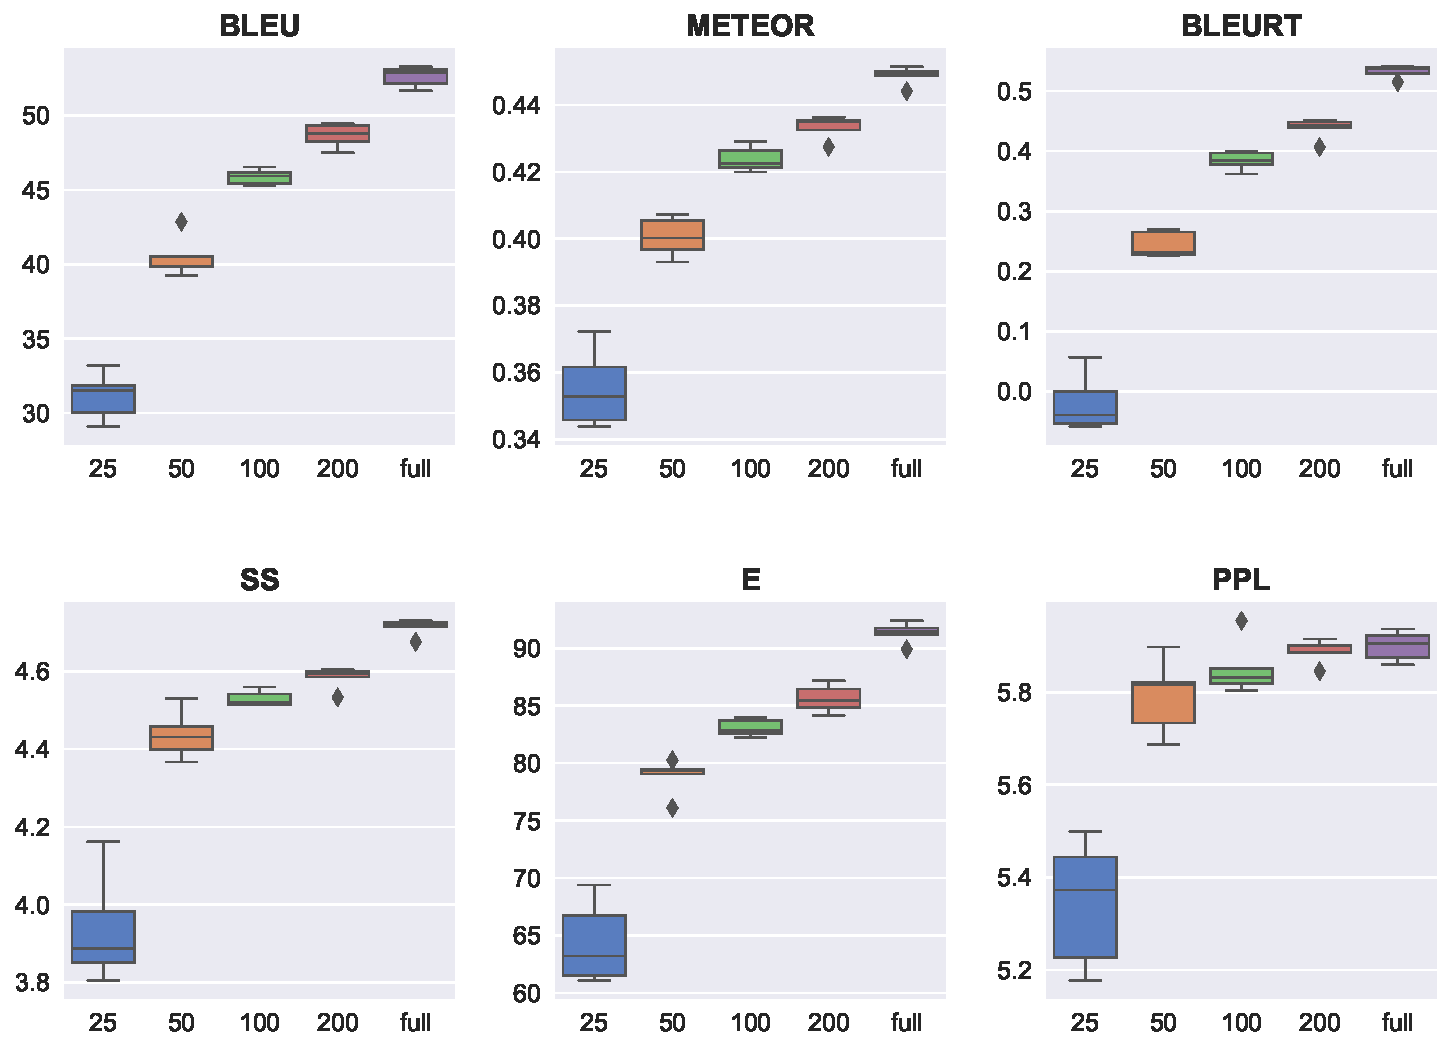
\includegraphics[width=\textwidth]{img/rel2text-fewshot.pdf}
    \caption{Boxplots for selected metrics from \autoref{tab:rel2text:auto} w.r.t. the number of examples (displayed on the \textit{x}-axis, $\textit{full} = 1522$), taking into account variance from individual random seeds.}\label{fig:rel2text:fewshot}
\end{figure}

\subsection{Findings from Manual Error Analysis}


\begin{figure}[t]
    \centering
    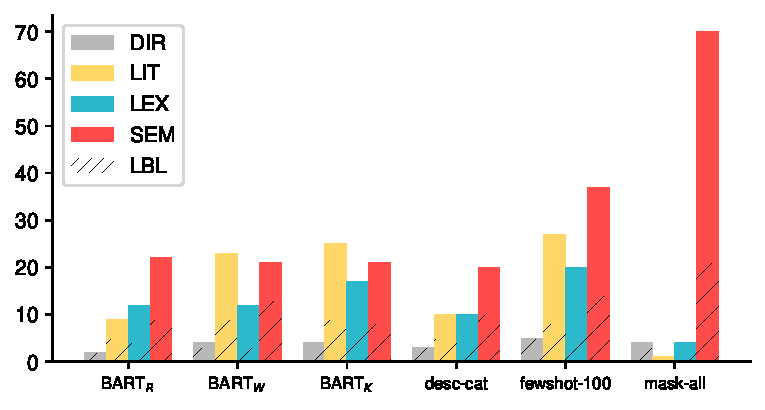
\includegraphics[width=0.7\textwidth]{img/rel2text-graph.pdf}
    \caption{Number of annotated errors per model (see \autoref{tab:rel2text:cat} for the description of error categories and \autoref{sec:rel2text:analysis} for the models). The striped part signifies that the label of the input was marked as unclear.}
    \label{fig:rel2text:manual}
\end{figure}
Results are summarized in \autoref{fig:rel2text:manual}; examples of model outputs for each error type are shown in \autoref{tab:rel2text:cat}.

\paragraph{Naturalness of Expressions} The \BARTk{} and \BARTw{} models use expressions that are too literal (\textsc{Lit}) in 23 and 29 cases, respectively, while the \BARTr{} and \textit{desc-cat} models do the same only in 11 cases (5 out of which are marked as \textsc{Lbl}, i.e., with an unclear label). This suggests that the variability of our dataset helps models to apply more natural expressions, especially if the relation is understandable from its label.

\paragraph{Semantic Errors} There is a near-constant portion of examples where the models make a semantic error (\textsc{Sem}) \textit{and} the input is marked as needing an extra description (\textsc{Lbl}). The models also make relatively many semantic errors, most prominently in the case of the \textit{fewshot-100} and the \textit{mask-all} models. The \textit{mask-all} model made a semantic error in 78 cases, suggesting that guessing the exact relation just from the entities is difficult (although still possible in 22 cases). Moreover, the outcomes from this model are fluent (only 4 \textsc{Lex} errors), making it hard to detect faulty cases.
The case of swapping the relation direction (\textsc{Dir}) is surprisingly not that common, which is probably down to having only a few examples in our dataset prone to this kind of error.

\paragraph{Additional Clues} There were only 12 out of 100 examples annotated as \textsc{Ent}, which suggests that the verbalization of the relation can be mostly decided irrespective of the entities in the triple. Notably, the results for \BARTr{} and \textit{desc-cat} are very similar, rendering the impact of extra descriptions negligible.


\subsection{Applications to Downstream Tasks}
\label{sec:rel2text:downstream}
Given that the \BARTr{} model can describe relations from their labels with high accuracy, we investigate if we can use the model to replace manually created templates in downstream tasks. We select two qualitatively different tasks, both using the idea of transforming individual input triples to simple sentences as a preprocessing step: tabular reasoning and zero-shot data-to-text generation.


\begin{table}[t]\centering
    \small
    \setlength{\tabcolsep}{4pt}
    \begin{tabular}{lcccc}\toprule
        \textbf{premise repr.}              & \textbf{dev} & $\alpha_1$ & $\alpha_2$ & $\alpha_3$ \\\midrule
        OPR \cite{gupta2020infotabs}        & 76.78        & 75.30      & 68.46      & 64.63      \\
        BPR \cite{neeraja2021incorporating} & 77.04        & 74.44      & 67.46      & 63.17      \\
        \BARTr{} (ours)                     & 74.44        & 74.31      & 64.59      & 63.46      \\
        \bottomrule
    \end{tabular}
    \caption{Accuracy for the dev set and test sets  $\alpha_{1,2,3}$ from the \textsc{InfoTabS} dataset. The results are averaged over 3 random seeds.}
    \label{tab:rel2text:nli}
\end{table}


\paragraph{Tabular Reasoning} For the task of \ac{nli} from a table, \citet{gupta2020infotabs} represent each table cell using a simple template \text{``The \textit{key} of \textit{title} are \textit{value}.''}. \citet{neeraja2021incorporating} extend their approach by preparing a fine-grained set of rules\footnote{Formalized using more than 250 lines of Python code: \url{https://github.com/utahnlp/knowledge\_infotabs/blob/main/scripts/preprocess/bpr.py\#L120}} for individual entity categories. We replicate the setup of \citet{neeraja2021incorporating} for the original (OPR) and better (BPR) paragraph representation using their public codebase. We then replace their templates with our \BARTr{} model, verbalizing the triple (\textit{title}, \textit{key}, \textit{value}). The results are summarized in Table \ref{tab:rel2text:nli}. Our manual evaluation suggests that the sentences from our model are indeed more grammatical (even compared to BPR), but we observe comparable performance across all three test sets. In line with \citet{mccoy2019right}, we conclude that for classification tasks such as NLI, the input content appears to be more important than the input form.


\begin{table}[t]\centering
    \small
    \setlength{\tabcolsep}{4pt}
    \begin{tabular}{clcccc}\toprule
        \textbf{dataset}                   & \textbf{model} & \textbf{BLEU} & \textbf{METEOR} & \textbf{O} & \textbf{H} \\\midrule
        \multirow{2}{*}{\textit{filtered}} & orig           & 43.19         & 39.13           & 0.152      & 0.073      \\
                                           & \BARTr{}       & 45.39         & 38.97           & 0.056      & 0.161      \\\cdashlinelr{1-6}
        \multirow{2}{*}{\textit{full}}     & orig           & 42.92         & 39.07           & 0.051      & 0.148      \\
                                           & \BARTr{}       & 44.63         & 38.93           & 0.058      & 0.166      \\
        \bottomrule
    \end{tabular}
    \caption{Lexical similarity metrics (BLEU, METEOR) and ommission (O) and hallucinaton (H) rate; following the setup in \citet{kasner2022neural}.}\label{tab:rel2text:zeroshot}
\end{table}

\paragraph{Zero-shot Data-to-Text Generation} In \autoref{sec:pipeline}, we described our approach for zero-shot D2T generation which requires transforming individual triples into text \cite{kasner2022neural}. Here, we replicate the setup on the WebNLG dataset, applying the \BARTr{} model instead of the templates. The results are summarized in Table \ref{tab:rel2text:zeroshot}.  We note that the pipeline using our model for preprocessing is able to achieve improvements of $\sim$2 BLEU points, at the cost of a slightly higher omission and hallucination rate, but crucially without needing the manual effort to create templates. A cursory examination shows that sentences produced by our model are qualitatively similar to the manual templates but more varied. Unlike the templates, our model may verbalize a relation differently depending on the context.
Overall, we argue that training a PLM on verbalizing individual relations can potentially replace the manual effort of creating simple templates, which will have a notable impact on scaling similar approaches to larger datasets.



\ZK{TODO: discuss ASPIRO: Any-shot Structured Parsing-error-Induced ReprOmpting for Consistent Data-to-Text Generation}


\section{Data-to-Text Generation with Large Language Models}
\label{sec:quintd}

\begin{refbox}
    This section is based on the paper \emph{Beyond Basic Benchmarks: Evaluating Open LLMs on Data-to-Text Generation} \cite{kasnerReferenceBasedMetricsAnalyzing2024}, joint work with Ondřej Dušek. The work \ZK{TODO}
\end{refbox}

% We analyze the behaviors of open \acp{llm} on the task of \ac{d2t} generation. To avoid the issue of \ac{llm} training data contamination with standard benchmarks, we design \datatool{} -- a tool for collecting novel structured data records from public APIs. Using a dataset collected with \datatool and leveraging reference-free evaluation, we analyze model behaviors on five D2T generation tasks.
% We find that recent open \acp{llm} (Llama2, Mistral, and Zephyr) can generate fluent and coherent text from standard data formats in zero-shot settings. However, we also show that the semantic accuracy of the outputs is a major issue: both according to our GPT-4-based metric and human annotators, more than 80\% of the outputs of open \acp{llm} contain a semantic error. We publicly release the code, data, and model outputs at \url{https://d2t-llm.github.io/}.


% Large language models (\acp{llm}; \citealp{ouyang2022TrainingLM,touvron2023llama,touvronLlamaOpenFoundation2023,jiangMistral7B2023,tunstallZephyrDirectDistillation2023}) have already left a mark in many areas of natural language processing (NLP). Surprisingly, their applicability to the task of data-to-text (D2T) generation \cite{reiter1997building,gatt2018survey} remains underexplored, with limited evaluation on a handful of well-established benchmarks only \cite{axelssonUsingLargeLanguage2023,yuanEvaluatingGenerativeModels2023}. Generating text from structured data is arguably challenging for \acp{llm}, given the specifics of D2T generation, such as long inputs, complex non-linear structure, and strict requirements on semantic accuracy. However, a more significant issue is perhaps the lack of testing grounds. The current D2T generation benchmarks are not only getting saturated \cite{vanmiltenburgBarriersEnablingFactors2023}, but also promote optimization towards traditional reference-based evaluation metrics, which were shown to correlate poorly with human judgment \cite{gehrmann2022repairing,vanderleeHumanEvaluationAutomatically2021,novikovaWhyWeNeed2017}. When it comes to the models, using closed \acp{llm} \cite{openai2023gpt4,chatgpt} is increasingly considered a bad research practice due to its non-reproducibility \cite{rogers2023closed,chen2023chatgpt}. On top of that, contamination of \ac{llm} training data with standard benchmarks further restricts the space for experiments \cite{golchin2023time,aiyappa-etal-2023-trust,balloccu2024leak}.


% In this paper, we propose an approach that allows us to analyze model behavior in D2T generation on novel, real-world structured data records with reference-free evaluation metrics. We begin by realizing that \textit{unlabeled data are plentiful}. To leverage the data for our experiments, we introduce \datatool\footnote{\underline{Q}uintet of \underline{U}nlabeled \underline{I}nputs for \underline{N}atural \underline{T}asks in \underline{D}ata-to-text, pronounced as ``quintet''} -- a tool for collecting structured data from five domains in standard formats: JSON,
% % \footnote{\url{https://www.json.org/}}
% CSV,
% % \footnote{\url{https://tools.ietf.org/rfc4180}}
% and Markdown.
% % \footnote{\url{https://www.rfc-editor.org/rfc/rfc7763.html}
% We choose the domains so that the data can be directly used as input for five distinct D2T generation tasks. Specifically, our tasks include generating weather forecasts, sports reports, product descriptions, chart captions, and entity descriptions (see Table \ref{tab:data}).
% %
% Next, we collect a set of 1,000 inputs with \datatool and use the inputs as an ad-hoc benchmark (called \benchmark) for testing the abilities of \acp{llm} for D2T generation. We assume that the data formats in \benchmark are common in the \acp{llm}' pretraining corpora, so we specify the task using instructions instead of standard finetuning with human-written outputs, capitalizing on the zero-shot abilities of instruction-tuned \acp{llm} (§\ref{sec:data}).


% We push towards better reproducibility by \textit{focusing on open \acp{llm}}, which -- apart from being more accessible -- also achieve increasingly better results across tasks \cite{zheng2023judging,open-llm-leaderboard}. For our experiments, we use three open \acp{llm} with 7B parameters: Llama-2 \cite{touvronLlamaOpenFoundation2023,llama-2-7b-32k}, Mistral \cite{jiangMistral7B2023}, and Zephyr \cite{tunstallZephyrDirectDistillation2023}. We also use GPT-3.5 \cite{chatgpt} as a closed model baseline for the final experiments. Given the behavioral nature of the experiments with \acp{llm} \cite{holtzmanGenerativeModelsComplex2023}, we put emphasis on reporting model behavior throughout the process  (§\ref{sec:experiments}).

% Another piece of the puzzle is \textit{reference-free evaluation}: using the input data as a ground for comparison instead of human references (§\ref{sec:eval}).
% % \cite{duvsek2017referenceless} 
% For evaluation, we use manual annotations from human crowdworkers \cite{vanderleeHumanEvaluationAutomatically2021}, along with a customized automatic metric based on GPT-4 \cite{liuGEvalNLGEvaluation2023,chiang-lee-2023-large,kocmiGEMBAMQMDetectingTranslation2023}. To get a fine-grained picture of model errors, we annotate semantic accuracy errors on the level of individual tokens \cite{thomsonGoldStandardMethodology2020,thomson2023evaluating}.

% Based on our results, we provide general recommendations about D2T generation with open \acp{llm} across tasks and formats (§\ref{sec:discussion}). Our main findings are as follows:
% \begin{itemize}
%     \item \textbf{Open \acp{llm} can generate fluent outputs from structured data} in common formats under zero-shot settings.
%     \item \textbf{Semantic accuracy is a major obstacle}: both human annotators and GPT-4-based metric report that over 80\% of outputs of open \acp{llm} on our data contain a semantic error.
%     \item \textbf{Long data inputs cause practical issues}, including the need for long-context models, increased GPU memory requirements, and unavailability of few-shot approaches.
%     \item \textbf{Outputs can be empirically improved by following several rules-of-thumb} for preprocessing the model input, such as including units, removing unnecessary fields, or prefixing the model answer.
% \end{itemize}


% \section{Reference-Free D2T Generation}
% \label{sec:data}

% \paragraph{Data Collection Tool}
% \label{sec:data_collection}
% We introduce a tool named \datatool{} for collecting ad-hoc test sets using public APIs in five different domains, and we collect one such set (\benchmark) for our experiments. Our main reasons for departing from the traditional scheme of benchmarking on well-established datasets are:
% \begin{enumerate}
%     \item Any published test sets may be potentially included in the training data of \acp{llm}.
%     \item Public sources of structured data offer enough resources for creating ad-hoc test sets.
%     \item Without human references, our data collection scheme is lightweight and replicable.
% \end{enumerate}

% Given the available public sources of data, we settled on the five tasks which are described in Table \ref{tab:data} (see Appendix \ref{app:data} for more details). The tasks are based on structured data in common formats: JSON, CSV, and Markdown.


% \begin{figure}[t]
%     \centering
%     \small
%     \textbf{Prompt}
%     \begin{verbatimbox}
%         Based on the given data:

%         \`{}\`{}\`{}

%         \{DATA\}

%         \`{}\`{}\`{}

%         Your task is to write a brief, fluent, and
%         coherent single-paragraph \{output\_type\} in natural
%         language. The text should be balanced and neutral.
%         Make sure that all the facts mentioned in the text
%         can be derived from the input data, do *not* add
%         any extra information.
%     \end{verbatimbox}
%     \textbf{Output prefix}
%     \begin{verbatimbox}
%         Sure! Here is the \{output\_type\}:

%         "
%     \end{verbatimbox}
%     \caption{The prompt $\mathcal{P}$ and the model output prefix we used for the experiments in this paper. \texttt{DATA} is filled with the data record  $x$ and \texttt{output\_type} is filled accordingly for each domain $\mathcal{D}$ (see Table \ref{tab:data}).}
%     \label{fig:quintd:prompt}
% \end{figure}


% \paragraph{\benchmark Dataset}
% \label{sec:dataset}
% The benchmark we collected using \datatool{} for our experiments in this paper (\datatool{}-1) contains 500 examples in the development set and 500 examples in the test set (100 examples per domain for each split). We keep the size of the dataset moderate for a quick experimental turnaround.

% We downloaded the data between November 2023 and January 2024. Note that the dataset contains only \textbf{unlabeled} data without any reference outputs (e.g., weather data, but not a textual weather forecast). New versions of the benchmark can be easily generated with the \datatool{} tool we provide.



% \paragraph{Task Definition}
% Each example in \benchmark consists of a structured data record $x$ from a domain $\mathcal{D} \in $ \{\texttt{openweather}, \texttt{gsmarena}, \texttt{ice\_hockey}, \texttt{owid}, \texttt{wikidata}\}. Given $x$ and a prompt $\mathcal{P}$, the goal is to generate natural language output $y$ faithful to the data $x$, according to the instructions in the prompt $\mathcal{P}$ (see Figure \ref{fig:prompt}).




% % Since diversity and controllability of the output style is generally an underexplored topic in D2T generation (although see \citealp{hanGeneratingDiverseDescriptions2021}; \citealp{perlitzDiversityEnhancedTabletoText2022}), we cover three scenarios with different prompts, focusing on \textit{stylized} and \textit{topic-centric generation}:
% % \begin{itemize}
% %   \item $\mathcal{P}_\text{direct}$ -- Generating \texttt{output\_type} in a neutral and balanced way.
% %   \item $\mathcal{P}_\text{stylized}$ -- Generating \texttt{output\_type} written in a specific style (\texttt{style}).
% %   \item $\mathcal{P}_\text{topic-centric}$ -- Generating \texttt{output\_type} focusing on a given aspect (\texttt{aspect}).
% % \end{itemize}

% % We selected the values of the style and aspect variables manually for each domain to accomodate for their specific purposes and data formats (see Table~\ref{tab:setups}).


% \section{Experiments}
% \label{sec:experiments}
% \paragraph{Experimental Process}
% \label{sec:process}
% Our goal is to avoid extensive data preprocessing and prompt engineering since these steps could harm the reproducibility and generalizability of our experiments. With this goal in mind, we decided to use the same prompt template $\mathcal{P}$ for all the domains and models.

% For a set of preliminary experiments, we first wrote down the initial version of the prompt and used the data without further preprocessing.
% We then iteratively improved our experimental setup by observing outputs on the development set.
% We describe all the observations and modifications we made before generating the final outputs on the test set in §\ref{sec:observations}.

% % https://drive.google.com/file/d/1vMj_to9BHdeX0BgD2eX_rN--Q2kl2uct/view?usp=sharing
% \begin{figure*}[ht]
%     \centering
%     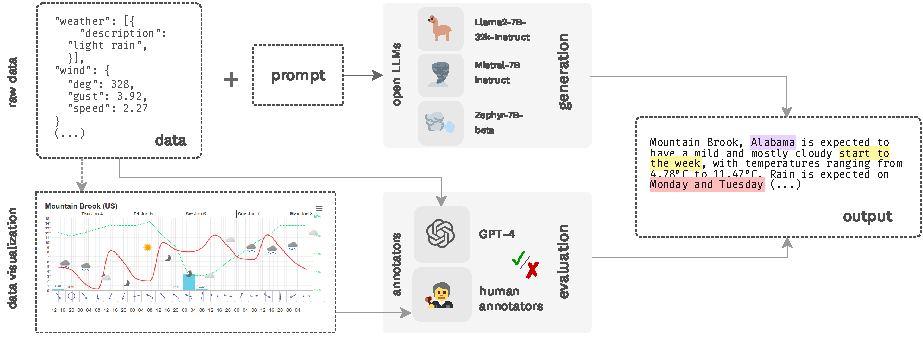
\includegraphics[width=\textwidth]{img/quintd_process.pdf}
%     \caption{Our experimental setup. We first generate the outputs using \acp{llm} that are given raw data and a task-specific prompt. We annotate the token-level semantic errors in the \ac{llm} outputs with (a) an automatic metric based on GPT-4 that matches the output to the raw data, and (b) human annotators, who annotate the errors in the output given the data visualization.}\label{fig:process}
% \end{figure*}

% \paragraph{Models}
% \label{sec:models}
% For our experiments, we selected the following \acp{llm} available under an open license:

% \begin{itemize}
%     \item \textbf{Llama2} \cite{touvron2023llama,llama-2-7b-32k},\\ \texttt{\small together\-computer\-/Llama-2-7B\--32K-Instruct}
%     \item \textbf{Mistral} \cite{jiangMistral7B2023},\\ \texttt{\small mistralai/Mistral-7B-Instruct-v0.1}
%     \item \textbf{Zephyr}  \cite{tunstallZephyrDirectDistillation2023}. \\ \texttt{\small HuggingFaceH4/zephyr-7b-beta}
% \end{itemize}

% The models are instruction-tuned, operate with 32k context, and perform well on recent benchmarks. All the models have 7B parameters and thus fit on a single NVIDIA A40 (48G VRAM) in 16-bit precision.  The models are available through HuggingFace \cite{wolf2019huggingface}.

% We accessed the models via an API provided by the \texttt{text-generation-webui} framework\footnote{\url{https://github.com/oobabooga/text-generation-webui}} running locally.
% For the final experiments, we also included GPT-3.5 (\texttt{gpt-3.5-turbo-1106}) accessed through the OpenAI API \cite{chatgpt}.

% \paragraph{Observations from Preliminary Experiments}
% \label{sec:observations}
% During development, we made several observations which we took into account for our final experimental setup:

% \paragraph{Any input field may appear in the output.} The models do not always select the most relevant fields for the given output. For example, we observed that the models commonly mention identifiers, timestamps, files, and other metadata, leading to unnatural outputs. Due to this, we decided not to include these irrelevant fields in the input.

% \paragraph{Units need to be specified explicitly.} If the units are not specified in the data record, the models tend to resort to their best guess. This may go unnoticed if the unit is evident from the context (e.g., the model will usually not report the temperature in Fahrenheit instead of Celsius), but it may get problematic if the value is ambiguous (e.g., wind speed in km/h versus m/s). Therefore, we explicitly add units to all data records where appropriate.

% \paragraph{Understandable labels are enough.} On the flip side, we decided not to add extra descriptions to the keys if the key was understandable from the label (e.g., \texttt{homeTeam} or \texttt{dimensions}). As discussed by \citet{kasner2023mind}, pretrained models tend to interpret the fields correctly as long as the label is human-readable. We only decided to include chart metadata for the CSV files in the \texttt{owid} domain.

% \paragraph{Long inputs can be troublesome.} The inputs in some domains can easily get longer than 10-20k tokens. This issue is amplified by the fact that the evaluated \acp{llm} tokenize numbers into individual digits. To accommodate for the long inputs, we picked models that accept up to 32k tokens.\footnote{For this reason, we use Llama-2-7B-32k with 32k token context \cite{llama-2-7b-32k} instead of the official Llama-2-7B-Instruct, which only supports 4k context \cite{touvronLlamaOpenFoundation2023}.} However, with long inputs, the GPU memory consumption also gets considerably higher, so we needed to downsample the data in \texttt{owid} and \texttt{openweather} to keep their length under \textasciitilde 8k tokens.


% \paragraph{Few-shot experiments are infeasible.} Due to the context-length limitations described above, we were not able to conduct few-shot experiments since we could not robustly fit an additional ($x_\text{example}$, $y_\text{example}$) pair in the prompt. We attempted to include only $y_\text{example}$ (making the setup ``half-shot''), but we observed that the models then tended to use entities from the example (unrelated to the actual input) in their outputs. Therefore, we decided not to follow this line of experiments (see §\ref{sec:future} for discussion).

% \paragraph{Deterministic decoding and sampling are on par.} In our preliminary experiments, we observed a roughly similar output quality for both deterministic decoding and sampling.\footnote{We used the \texttt{text-generation-webui} default decoding parameters: \texttt{temperature}=0.7, \texttt{top\_p}=0.9, and \texttt{top\_k}=20.} For the final experiments, we decided to use deterministic decoding, which is non-parametric and conceptually more suitable for D2T generation.

% \paragraph{Prefixing the output makes parsing easier.} Even with variations of a \textit{``generate only the output''} instruction appended to the prompt, the models (especially Llama2) tended to first confirm the request. For that reason, we decided to prefix the input for all the models with \textit{``Sure! Here is the \{output\_type\}: "''}. The opening quote at the end of the prefix allowed us to robustly parse the text simply by stripping the closing quote from the model output.

% \paragraph{The outputs are fluent but inaccurate.} We observed that the vast majority of model outputs were grammatically and stylistically correct, capturing the output type specified in the prompt. However, we also noticed that the outputs contained many factual errors (even after emphasizing the focus on factual accuracy in the prompt, see Figure \ref{fig:prompt}). This observation led us to evaluate the model outputs using token-level annotations focused on semantic accuracy errors \cite{reiterSharedTaskEvaluating2020}.



% \paragraph{Final Experiments}
% \label{sec:basic}

% Taking the observations in §\ref{sec:observations} into account, we proceeded to generate the outputs on the test set of \benchmark for token-level error analysis. We first preprocessed the data as mentioned: we stripped out unnecessary fields, added units, and downsampled the data to fit the context. For all the models mentioned in §\ref{sec:models}, we used the prompt in Figure \ref{fig:prompt} and deterministic decoding with a maximum length of 512 tokens.

% For comparison, we also generated outputs for the same inputs and identical prompts with GPT-3.5.\footnote{We did not include GPT-3.5 in our preliminary experiments since closed models are not our focus. We also did not use GPT-4 because we reserve the model for evaluation; see §\ref{sec:gpt4eval}.} Note that even though we fixed the temperature and seed to $0$, the rest of the decoding parameters are inaccessible to us and may differ from the parameters we used for the open models.





% \section{Evaluation}
% \label{sec:eval}
% For evaluation, we focus on \textit{semantic accuracy} errors. We compare the generated texts to the input data, looking for parts of texts that are not faithful to the input data. We annotate the errors on the token level, considering all the tokens in the output text as potential sources of errors.

% Regarding the error taxonomy, we settled on four error categories: \errinc{INCORRECT}, \errnc{NOT\_CHECKABLE}, \errmis{MISLEADING}, and \errother{OTHER}. The taxonomy is inspired by the methodology discussed in \citet{thomsonGoldStandardMethodology2020} and \citet{thomson2023evaluating}. To keep the annotation tractable, we decided not to distinguish between fine-grained categories (e.g., \textit{incorrect name} vs. \textit{incorrect number}). The descriptions of our error categories, as presented in the instructions for annotation, are included in Table \ref{tab:errors}.

% \begin{table*}[t]
%     \small
%     \centering
%     \begin{tabular}{p{2.25cm}p{12.5cm}} \toprule                                                                                        \\
%         \textbf{Error}         & \textbf{Description}                                                                        \\ \midrule
%         \errinc{INCORRECT}     & The fact in the text contradicts the data.                                                  \\
%         \errnc{NOT\_CHECKABLE} & The fact in the text cannot be checked given the data.                                      \\
%         \errmis{MISLEADING}    & The fact in the text is misleading in the given context.                                    \\
%         \errother{OTHER}       & The text is problematic for another reason, e.g., grammatically or stylistically incorrect,
%         irrelevant, or repetitive.                                                                                           \\\midrule

%         \textbf{Example}       &                                                                                             \\

%         \textit{data}          &
%         \textbf{Nokia 3310} |
%         \textit{color}: black, blue, grey |
%         \textit{display}: 320x240px                                                                                          \\
%         \textit{text}          &
%         Nokia 3310 is \errnc{produced in Finland} and features a \errinc{320x320} display. It is \errmis{misleading}{available in black color}. \errmis{other}{The data seem to provide only partial information about the phone.}
%         \vspace*{0.1cm}
%         \\ \bottomrule
%         % \textit{explanation}                             &
%         % \begin{description}[nosep]\item[produced in Finland] The country where the phone is produced is not mentioned in the data.
%         %   \item[320x320] The data mentions that the display has resolution 320x240px.
%         %   \item[available in black color] Misleadingly suggests that the phone is not available in other colors.
%         %   \item[The data seem to provide (...)] The note is irrelevant for the phone description.      \end{description}                                                                                                                                                                                                                                   \\\bottomrule
%     \end{tabular}
%     \caption{Categories of errors annotated in our evaluation and an example demonstrating the error types. See Appendix \ref{app:humeval} for an explanation of individual errors in the example.}
%     \label{tab:errors}
% \end{table*}

% We employ two complementary evaluation schemes:
% \begin{itemize}
%     \item \gptmetric{}: \textbf{an automatic metric} based on GPT-4 (§\ref{sec:gpt4eval}),
%     \item \humanmetric{}: \textbf{human evaluation} based on crowdsourcing (§\ref{sec:humaneval}).
% \end{itemize}

% These two schemes are based on similar instructions and produce (nearly) equivalent outputs. The main idea in introducing multiple schemes is to compensate for the shortcomings of each approach and thus increase the replicability and robustness of our results.


% \paragraph{GPT-4-based Evaluation}
% \label{sec:gpt4eval}

% \ac{llm}-based metrics can be customized for a particular task without the need for training data. For our experiments, we employ a metric based on GPT-4 (\texttt{gpt-4-1106-preview}, \citealp{openai2023gpt4}), which was shown to be superior in following fine-grained instructions compared to other \acp{llm} and to have high correlations with human judgment on evaluating generated texts  \cite{zhaoInvestigatingTabletoTextGeneration2023,sottanaEvaluationMetricsEra2023,kocmiGEMBAMQMDetectingTranslation2023,kocmiLargeLanguageModels2023}.
% % Compared to using fine-tuned models for token-level evaluation \cite{kasnerTextinContextTokenLevelError2021}, this allows us to customize the metric for a particular task without the need for training data.

% \gptmetric{} is instantiated using a prompt and a system message describing the task. We instruct the model to produce a JSON output with sequentially ordered errors using the following format:

% \small
% \begin{verbatim}
% {
%   "errors": [{
%     "reason": [REASON],
%     "text": [TEXT_SPAN],
%     "type": [ERROR_CATEGORY]
%     }, 
%     ...]
% }.
% \end{verbatim}
% \normalsize


% Note that we require that the model first generates the free-form text \textit{reason} for the error. Generating the reason incurs almost no extra cost, and our cursory observations suggest that requiring it leads to more precise outputs.

% Concerning the alignment of the model outputs with the original text, we perform matching on \texttt{TEXT\_SPAN}. We ensure that the model response is a valid JSON using OpenAI's \texttt{response\_format} parameter.  See Appendix \ref{app:gpt4eval} for more details about the metric, including the prompt and the system message.


% \paragraph{Human-based Evaluation}
% \label{sec:humaneval}

% An automatic metric based on a closed \ac{llm} makes the evaluation potentially non-reproducible and biased \cite{kocmiGEMBAMQMDetectingTranslation2023,wangLargeLanguageModels2023}, for which we compensate by obtaining annotations from human annotators.

% For the human annotation metric \humanmetric{}, we prepared a custom web interface
% %  based
% %%% TODO %%% 
% % \OD{remove cite for anonymized version?}
% %%% %%% 
% % on \textsc{TabGenie} \cite{kasner2023tabgenie}, 
% where an annotator is able to annotate a text span with a selected error category. We created custom visualizations for each data format. Unlike with \gptmetric{}, we did not ask the crowdworkers for free-form reasoning about the errors since that would make the annotation more complex.

% We hired annotators on the Prolific crowdsourcing platform.\footnote{\url{https://prolific.com}} In total, we hired 100 annotators, each annotating 20 examples (4 model outputs for each of the five domains). We selected annotators with at least 10 completed tasks and a 100\% approval rate, having English as their primary language. We paid the annotators \textsterling 9 per hour, according to the platform's recommendations. The median time for completing the annotations was 47 minutes. See Appendix \ref{app:humeval} for the instructions for the annotators and the annotation interface and Appendix \ref{app:outputs} for the data visualizations.




% % \paragraph{Evaluating Controllability}

% % Due to our resource limitations, we were not able to run the token-level error annotations for all the stylized outputs. Instead, we randomly selected 10 outputs for each domain on which we run the GPT-4 annotations, and two annotators (authors of the paper) rated the adherence to style along with free-form comments.

% \section{Results and Discussion}
% \label{sec:discussion}

% A summary of the token-level annotations is in Table \ref{tab:results_agg} and \ref{tab:results_errperex}, with detailed results per domain provided in Appendix \ref{app:full_results}.


% \begin{table*}[ht]
%     \small
%     \centering
%     \begin{tabular}{lccccccccccr}
%         \toprule
%                          & \multicolumn{2}{c}{\textbf{Incorrect}} & \multicolumn{2}{c}{\textbf{Not Checkable}} & \multicolumn{2}{c}{\textbf{Misleading}} & \multicolumn{2}{c}{\textbf{Other}} & \multicolumn{2}{c}{\textbf{All categories}} &                                                                                                     \\
%                          & \gptmetric{}                           & \humanmetric{}                             & \gptmetric{}                            & \humanmetric{}                     & \gptmetric{}                                & \humanmetric{} & \gptmetric{}  & \humanmetric{} & \gptmetric{}  & \humanmetric{} & \# \textbf{Tok.} \\\midrule

%         \textbf{Llama2}  & \textbf{2.46}                          & 1.57                                       & 0.90                                    & 1.25                               & \textbf{0.20}                               & 0.25           & 0.13          & \textbf{0.10}  & 3.70          & 3.18           & 83.8             \\
%         \textbf{Mistral} & 2.80                                   & 2.03                                       & 0.52                                    & 1.12                               & 0.37                                        & 0.44           & 0.11          & 0.25           & 3.80          & 3.85           & 114.9            \\
%         \textbf{Zephyr}  & 2.50                                   & \textbf{1.44}                              & \textbf{0.40}                           & \textbf{0.77}                      & 0.39                                        & \textbf{0.20}  & \textbf{0.06} & 0.16           & \textbf{3.35} & \textbf{2.58}  & 98.0             \\ \cdashlinelr{1-12}
%         \textbf{GPT-3.5} & 1.57                                   & 0.65                                       & 0.32                                    & 0.49                               & 0.42                                        & 0.18           & 0.02          & 0.07           & 2.32          & 1.39           & 84.9             \\ \bottomrule
%     \end{tabular}
%     \caption{The average \textit{numbers of errors per output} (lower is better) based on GPT-4 (\gptmetric{}) and human annotators (\humanmetric{}). We also include the average number of tokens per output in the rightmost column. The results of the best open \ac{llm}  are emphasized.}
%     \label{tab:results_agg}
% \end{table*}


% \begin{table*}[ht]
%     \small
%     \centering
%     \begin{tabular}{lcccccccccc}
%         \toprule
%                          & \multicolumn{2}{c}{\textbf{Incorrect}} & \multicolumn{2}{c}{\textbf{Not Checkable}} & \multicolumn{2}{c}{\textbf{Misleading}} & \multicolumn{2}{c}{\textbf{Other}} & \multicolumn{2}{c}{\textbf{All categories}}                                                                                    \\
%                          & \gptmetric{}                           & \humanmetric{}                             & \gptmetric{}                            & \humanmetric{}                     & \gptmetric{}                                & \humanmetric{} & \gptmetric{}  & \humanmetric{} & \gptmetric{}  & \humanmetric{} \\\midrule
%         \textbf{Llama2}  & 0.78                                   & 0.53                                       & 0.46                                    & 0.57                               & \textbf{0.15}                               & 0.17           & 0.09          & \textbf{0.08}  & 0.92          & 0.86           \\
%         \textbf{Mistral} & 0.78                                   & 0.54                                       & 0.32                                    & 0.50                               & 0.23                                        & 0.21           & 0.08          & 0.14           & 0.93          & 0.81           \\
%         \textbf{Zephyr}  & \textbf{0.77}                          & \textbf{0.47}                              & \textbf{0.26}                           & \textbf{0.42}                      & 0.27                                        & \textbf{0.16}  & \textbf{0.04} & 0.12           & \textbf{0.88} & \textbf{0.76}  \\\cdashlinelr{1-11}
%         \textbf{GPT-3.5} & 0.64                                   & 0.38                                       & 0.21                                    & 0.29                               & 0.26                                        & 0.13           & 0.02          & 0.06           & 0.75          & 0.61           \\ \bottomrule
%     \end{tabular}
%     \caption{The ratio of \textit{outputs containing at least one error} (lower is better) based on GPT-4 (\gptmetric{}) and human annotators (\humanmetric{}). The results of the best open \ac{llm}  are emphasized.}
%     \label{tab:results_errperex}
% \end{table*}



% \paragraph{How Accurate Are the Model Outputs?}
% Depending on the model, between 74-85\% of examples contain an error according to \humanmetric, suggesting that open \acp{llm} make semantic errors very often. According to \gptmetric, the number is as high as 88-93\%.

% The most common error type is \texttt{INCORRECT}. As shown in Table \ref{tab:results_agg}, all the open \acp{llm} make more than \textbf{two statements contradicting the data per output on average}. The \texttt{NOT\_CHECKABLE} errors are also relatively common: more than one per output on average according to \humanmetric, and at least one being present in more than 26\% of examples according to both metrics.

% The results vary widely according to the domain (see Appendix \ref{app:full_results}). For example, the outputs in \texttt{wikidata} contain much more \texttt{NOT\_CHECKABLE} errors on average (1.54 per output according to \humanmetric) than  \texttt{INCORRECT} errors (0.12 per output according to \humanmetric), suggesting that with simpler inputs, the models tend to introduce extra information. The \texttt{openweather} domain seems to be the most complex with the longest outputs (\textasciitilde 164 tokens), more than eight errors in the output on average, and >90\% of outputs containing an error.

% The differences between the open \acp{llm} are not major. Out of the open \acp{llm}, Zephyr has the best results across categories and metrics, followed by Llama2. However, the outputs of Mistral are longer on average, leaving more space for errors. GPT-3.5 (which we consider separately) does generally better according to both \gptmetric and \humanmetric, although it still makes an error in 60-75\% of examples (2 errors per example on average). In general, the results show that \acp{llm} make too many semantic errors to be usable in practice for D2T generation in a zero-shot setting.



% \paragraph{Do Evaluation Methods Agree?}
% \label{sec:metricscorr}
% To quantify the agreement of our evaluation metrics, we computed the Pearson correlation coefficient between the error counts on the level of tokens, examples, and domains (see Appendix \ref{app:corr} for details). The correlation on the level of tokens is weak ($r_{\text{token}}=0.26$) but gets better on the example-level ($r_{\text{example}}=0.55$) and even better on the domain-level ($r_{\text{domain}}=0.92$). In Table \ref{tab:errors_tokenlevel}, we show the percentage of tokens marked by individual metrics. The metrics agree on the specific tokens in less than 6\%, although they both mark around 21\% of tokens as erroneous.
% % , suggesting that the error spans may be subject to interpretation.

% We also measure inter-annotator agreement between human annotators. For that, we obtained annotations from two annotators for 100 model outputs. The results are similar: the annotators agree weakly on the token level ($r_{\text{token}}=0.36$), stronger on the example level ($r_{\text{example}}=0.53$), and even stronger on the domain level ($r_{\text{domain}}=0.85$). We conclude that while the details regarding error spans and categories may vary, the annotators as well as GPT-4 generally agree on the accuracy of model outputs for a given set of examples. In the future, the agreement could be improved by measuring errors on the phrase level \cite{vamvas2022little}.

% % The results show that while \gptmetric and \humanmetric do not agree much on individual token spans, they correlate well for high-level ranking of the models.

% \begin{table}[t]
%     \small
%     \centering
%     \begin{tabular}{lccc}
%         \toprule
%         {}                       & \gptmetric{} & \humanmetric{} & \gptmetric{} + \humanmetric{} \\
%         \midrule
%         \bfseries Incorrect      & 0.135        & 0.099          & 0.040                         \\
%         \bfseries Not checkable  & 0.039        & 0.076          & 0.016                         \\
%         \bfseries Misleading     & 0.022        & 0.022          & 0.001                         \\
%         \bfseries Other          & 0.008        & 0.018          & 0.001                         \\
%         \bfseries All categories & 0.204        & 0.214          & 0.059                         \\
%         \bottomrule
%     \end{tabular}
%     \caption{The ratio of \textit{tokens marked as erroneous} by GPT-4 (\gptmetric), human annotators (\humanmetric), and both metrics at the same time (\gptmetric + \humanmetric).}
%     \label{tab:errors_tokenlevel}
% \end{table}


% % \begin{table}[t]
% %   \small
% %   \centering
% %   \begin{tabular}{lrrrr}
% %     \toprule
% %                & \gptmetric{} & \humanmetric{} & \textbf{Both} & \textbf{None} \\
% %     \midrule
% %     Total (\%) & 11.68        & 12.72          & 5.88          & 66.89         \\    \bottomrule
% %   \end{tabular}
% %   \caption{Percentage of tokens annotated with an error (of any category) by GPT-4 (only), human annotators (only), both metrics at the same time, or none of the metrics.}
% % \end{table}


% \paragraph{Recommendations and Directions}
% \label{sec:future}
% \paragraph{Forget fluency, solve accuracy.} The output of \acp{llm} is satisfactory regarding the style, format, and purpose of the text. However, the amount of semantic errors remains very high. Improving the semantic accuracy of the models
% %%% TODO %%%
% % \OD{remove Pat's cite for anonymization} \cite{schmidtova2023semantic}
% %%% %%%
% \cite{li2022faithfulness}, along with new model-based evaluation metrics \cite{liuGEvalNLGEvaluation2023,xuINSTRUCTSCOREExplainableText2023}, could thus help to bring improve \ac{llm}-based D2T generation systems where it is most needed.



% \paragraph{Use efficient models.} The memory issues with long context, making few-shot experiments infeasible, can potentially be solved by using more efficient long-context models equipped with Flash Attention \cite{dao2022flashattention} and fast inference libraries such as \texttt{llama.cpp}.\footnote{\url{https://github.com/ggerganov/llama.cpp}} A potentially suitable open \ac{llm} in this respect is the long-context Llama2 (\citealp{xiong2023effective}; model to be released).


% \paragraph{Test the models in the wild.} Except for using an ad-hoc dataset of real-world data as we did in our work, the ecological validity of D2T evaluation can also be ensured by continuous evaluation with human users \cite{zheng2023judging} and evaluating the real-world impact of the systems \cite{reiter2023impact}.


% \paragraph{Multilinguality is an opportunity.}With the recent efforts in extending D2T generation to low-resource languages \cite{cripwell-etal-2023-2023}, multilingual D2T generation with open \acp{llm} seems a promising direction. Although we did not go beyond English, initial steps were already done by works such as \citet{lorandi2023data}.


% \paragraph{Be careful about subtle bugs.} During our preliminary experiments, we uncovered subtle bugs in API calls such as incorrect instruction templates\footnote{\url{https://huggingface.co/docs/transformers/chat_templating}} or involuntary input truncation. With the apparent ease of API access and robustness of \acp{llm}, such bugs could go unnoticed and artificially skew the model performance.




